\documentclass[prb,preprint]{revtex4-1} 
% The line above defines the type of LaTeX document.
% Note that AJP uses the same style as Phys. Rev. B (prb).

% The % character begins a comment, which continues to the end of the line.

\usepackage{amsmath}  % needed for \tfrac, \bmatrix, etc.
\usepackage{amsfonts} % needed for bold Greek, Fraktur, and blackboard bold
\usepackage{graphicx} % needed for figures
%\usepackage{epstopdf}

\begin{document}

% Be sure to use the \title, \author, \affiliation, and \abstract macros
% to format your title page.  Don't use lower-level macros to  manually
% adjust the fonts and centering.

\title{KAT-7 and Python as tools for teaching radio interferometry}
% In a long title you can use \\ to force a line break at a certain location.

\author{Daniel V. Schroeder}
\email{dschroeder@weber.edu} % optional
\altaffiliation[permanent address: ]{101 Main Street, 
  Anytown, USA} % optional second address
% If there were a second author at the same address, we would put another 
% \author{} statement here.  Don't combine multiple authors in a single
% \author statement.
\affiliation{Department of Physics, Weber State University, Ogden, UT 84408-2508}
% Please provide a full mailing address here.

\author{David P. Jackson}
\email{ajp@dickinson.edu}
\affiliation{Department of Physics, Dickinson College, Carlisle, PA 17013}

% See the REVTeX documentation for more examples of author and affiliation lists.

\date{\today}

\begin{abstract}
This article explains and illustrates the use of \LaTeX\ in preparing manuscripts
for submission to the American Journal of Physics (AJP). While it is not a
comprehensive reference, we hope it will suffice for the needs of most
AJP authors.
\end{abstract}
% AJP requires an abstract for all regular article submissions.
% Abstracts are optional for submissions to the "Notes and Discussions" section.

\maketitle % title page is now complete


\section{Introduction} % Section titles are automatically converted to all-caps.
% Section numbering is automatic.

\section{Fundamentals of Interferometry}

The phrase ``Fundamentals of Interferometry'' can refer to either a course or the ipython notebook based textbook which is used to teach the interferometry course. To distinguish between
these two concepts we will be making use of italic and bold formatting, i.e \textit{Fundamentals of Interferometry} refer to the course itself, while  
\textbf{Fundamentals of Interferometry} refer to the textbook the course uses. The official course website is: . The electronic textbook can be obtained here:

The \textit{Fundamentals of Interferometry} course differs from conventional interferometry courses in that it makes use of novel teaching mediums. We discuss this 
in greater detail in Section~\ref{sec:course_material}. Moreover, the \textit{Fundamentals of Interferometry} is also unique in terms of the physical content that it covers.
We describe the course content in more detail in Section~\ref{sec:course_content}.

\subsection{Course Material}
\label{sec:course_material}
\begin{figure}[h!]
% The bracketed code determines the figure's placement:  "h" stands for 
% "here", telling LaTeX to put the figure as close to the current location 
% as possible.  The ! overrides LaTeX's tendency to try to find a location 
% that it thinks is better.  But don't agonize over the exact figure placement 
% in your submitted manuscript.  For your initial submission, just make sure 
% each figure is reasonably close to where it's first referenced.
\centering
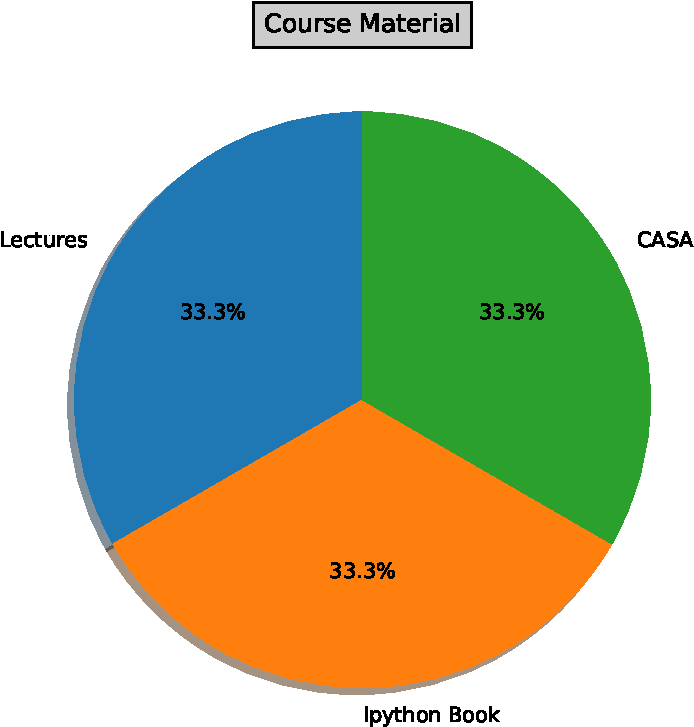
\includegraphics[width=0.7\textwidth]{./course_material.pdf}
\caption{The teaching mediums that is used in teaching \textit{Fundamentals of Interferometry} can be divided into three broad categories, namely conventional 
lectures, an ipython notebook based textbook and CASA. Each of these categories contribute an equal amount to the total body of teaching material.}
\label{gasbulbdata}
\end{figure}

In particular we make use of three teaching mediums:

\begin{enumerate}
 \item \textit{Conventional lectures}: We make use of conventional presentation style lectures. The course 
 consists of 32 hours of lecturing. The main focus of the lectures are to get the main interferometric concepts across. The finer details  
 can be obtained from the the text book. The lectures are also recorded and are made available to the students so that they can refer back to the material at any point.
 The presentations and the recorded lectures can be found on the official course website.
 \item \textit{Ipython notebook based textbook}: We make use of a novel text book in this course. It consists of ipython notebooks. The main drawback of a conventional 
 textbook is that complicated mathematical ideas are not supplemented with executable computer code. It is much easier to learn an abstract mathematical construct 
 if you can also inspect a small piece of executable code that also implements the idea. We address this short coming in the electronic book by providing 
 executable pieces of python code that implements most of the complicated ideas, making it easier to grasp and understand.
 \item \textit{\textsc{CASA}}: \textsc{CASA} is a reduction package. To grasp interferometry it is crucial for students to not only understand the theoretical concepts, but to also gain 
 practical experience in reducing real interferometric data. That is why each student is required to reduce a real KAT7 dataset as part of the course. KAT7 is a proof of concept instrument and can be used as a teaching tool. 
 Since we are making use of KAT7 data in this course students have access to real non-sensitive sceintific data which they may use to learn the basics. 
\end{enumerate}

\subsection{Course Content}
\label{sec:course_content}
The \textit{Fundamentals of Interferometry} course covers a lot of background material which is normally just 
skipped over as it is simply assumed that most of the students are familiar with the background material needed to study interferometry. We have found that, in particular for a South African context, this is not the case.
The students that partake in the course come from a wide variety of backgrounds including: Chemistry, Physics, Mathematics, Astronomy and Computer Science. Most of the students, therefore, do not have enough familiarity with all
the background topics required to understand interferometry. We spend about a third of the course teaching the required background topics.
Another important aspect of interferometry is to gain practical experience reducing interferometric data. We spend another third of the course on teaching students 
how to reduce real interferometric data. The remaining time is evenly allocated to the most important interferometric topics.

\subsubsection{Background Topics}
\label{sec:background_topics}
We cover the following background topics in some detail:

\begin{enumerate}
\item  \textit{Positional Astronomy}: In positional astronomy we explain different astronomical coordinate systems, in particular the equatorial and horizontal coordinate system, which are crucial for students to know if they hope 
to become proficient in interferometry. We also define concepts like hour angle and local sidereal time which are fundamental to 
to master if one wants to compute the $uv$-coverage of an array from first principals. We also cover the direction cosine coordinate system in some detail. This coordinate 
system is often used in interferometry, because using it automatically exposes a Fourier relationship between the sky brightness distribution and the measurements 
an interferometer makes, i.e visibilities.
\item {\textit}{}

\end{enumerate}







\appendix*   % Omit the * if there's more than one appendix.

\section{Uninteresting stuff}

Appendices are for material that is needed for completeness but
not sufficiently interesting to include in the main body of the paper.  Most
articles don't need any appendices, but feel free to use them when
appropriate.  This sample article needs an appendix only to illustrate how 
to create an appendix.


\begin{acknowledgments}

We gratefully acknowledge Harvey Gould and Jan Tobochnik, who created an earlier 
AJP \LaTeX\ sample article that inspired this one.  This work was supported by the 
American Association of Physics Teachers.

\end{acknowledgments}


\begin{thebibliography}{99}
% The numeral (here 99) in curly braces is nominally the number of entries in
% the bibliography. It's supposed to affect the amount of space around the
% numerical labels, so only the number of digits should matter--and even that
% seems to make no discernible difference.

\bibitem{latexsite} \LaTeX\ Project Web Site, \url{<http://www.latex-project.org/>}.

\bibitem{wikibook} \textit{\LaTeX} (Wikibook), \url{<http://en.wikibooks.org/wiki/LaTeX/>}.

\bibitem{latexbook}Helmut Kopka and Patrick W. Daly, \textit{A Guide to
\LaTeX}, 4th edition (Addison-Wesley, Boston, 2004).

\bibitem{revtex} REV\TeX\ 4 Home Page, \url{<https://authors.aps.org/revtex4/>}.

\bibitem{cloudLaTeX} On the other hand, you can avoid the installation process
entirely by using a cloud-based \LaTeX\ processor such as ShareLaTeX,
\url{<https://www.sharelatex.com/>}, or write\LaTeX, \url{<https://www.writelatex.com/>}.

\bibitem{nevermindlogic} In typography, aesthetics often takes precedence over logic.

\bibitem{FontEncodingComment} Please don't try to handle foreign characters 
and accents with the \texttt{inputenc} and \texttt{fontenc} packages, which 
are incompatible with AJP's editing process.

\bibitem{wikimathpage} See the Mathematics chapter of Ref.~\onlinecite{wikibook}
for an excellent overview of math symbols and equations, with examples.

\bibitem{labelnames} Thinking up a good label name takes a moment, but 
it's worth the trouble; we strongly advise against using labels like 
\texttt{eq2}, which become extremely confusing after you decide to add 
another equation before Eq.~(\ref{deriv}).

\bibitem{footnotes} You need to process a file twice to get the counters correct.

\bibitem{mermin} N. David Mermin, ``What's wrong with these equations?,'' 
Phys. Today \textbf{42} (10), 9--11 (1989).  
% Note that the issue number (10) in this citation is required, because
% each issue of Physics Today starts over with page 1.  Also note the use of
% an en-dash (--), not a hyphen (-), for the page range.

\bibitem{editorsite} American Journal of Physics Editor's Web Site, 
\url{<http://ajp.dickinson.edu>}.

\bibitem{feynman} Richard P. Feynman, Robert B. Leighton, and Matthew Sands, 
\textit{The Feynman Lectures on Physics, Vol.\ 1} (Addison-Wesley, 1964), p.~3-10.
% Note that this book is paginated by chapter; "3-10" is a single page reference
% that uses a hyphen, not a range of pages that would us an en-dash (--).

\bibitem{noBIBTeX} Many \LaTeX\ users manage their bibliographic data with 
a tool called BIB\TeX.  Unfortunately, AJP cannot accept BIB\TeX\ files; all 
bibliographic references must be incorporated into the manuscript file
as shown here, at least when you send an editable file for production.

\bibitem{dyson} Freeman J. Dyson, ``Feynman's proof of the Maxwell equations,''
Am. J. Phys. \textbf{58} (3), 209--211.  
% The issue number (3) in this citation is optional, because AJP's pagination 
% is by volume.

\bibitem{examplevolume} M. R. Flannery, ``Elastic scattering,'' in 
\textit{Atomic, Molecular, and Optical Physics Handbook}, edited by
G. W. F. Drake (AIP Press, New York, 1996), p.~520.

\bibitem{AIPstylemanual} \textit{AIP Style Manual}, 4th edition (American 
Institute of Physics, New York, 1990). Available online at 
\url{<http://www.aip.org/pubservs/style/4thed/toc.html>}. Although parts of 
it have been made out of date by advancing technology, most of this manual 
is still as useful as ever. Just be sure to follow AJP's specific rules
whenever they conflict with those in the manual.

\end{thebibliography}

% If your manuscript is conditionally accepted, the editors will ask you to
% submit your editable LaTeX source file.  Before doing so, you should move
% all tables and figure captions to the end, as shown below.  Tables come 
% first, followed by figure captions (with figure inclusions commented-out).
% Figures should be submitted as separate files, collected with the
% LaTeX file into a single .zip archive.

%\newpage   % Start a new page for tables

%\begin{table}[h!]
%\centering
%\caption{Elementary bosons}
%\begin{ruledtabular}
%\begin{tabular}{l c c c c p{5cm}}
%Name & Symbol & Mass (GeV/$c^2$) & Spin & Discovered & Interacts with \\
%\hline
%Photon & $\gamma$ & \ \ 0 & 1 & 1905 & Electrically charged particles \\
%Gluons & $g$ & \ \ 0 & 1 & 1978 & Strongly interacting particles (quarks and gluons) \\
%Weak charged bosons & $W^\pm$ & \ 82 & 1 & 1983 & Quarks, leptons, $W^\pm$, $Z^0$, $\gamma$ \\
%Weak neutral boson & $Z^0$ & \ 91 & 1 & 1983 & Quarks, leptons, $W^\pm$, $Z^0$ \\
%Higgs boson & $H$ & 126 & 0 & 2012 & Massive particles (according to theory) \\
%\end{tabular}
%\end{ruledtabular}
%\label{bosons}
%\end{table}

%\newpage   % Start a new page for figure captions

%\section*{Figure captions}

%\begin{figure}[h!]
%\centering
%\includegraphics{GasBulbData.eps}   % This line stays commented-out
%\caption{Pressure as a function of temperature for a fixed volume of air.  
%The three data sets are for three different amounts of air in the container. 
%For an ideal gas, the pressure would go to zero at $-273^\circ$C.  (Notice
%that this is a vector graphic, so it can be viewed at any scale without
%seeing pixels.)}

%\label{gasbulbdata}
%\end{figure}

%\begin{figure}[h!]
%\centering
%\includegraphics[width=5in]{ThreeSunsets.jpg}   % This line stays commented-out
%\caption{Three overlaid sequences of photos of the setting sun, taken
%near the December solstice (left), September equinox (center), and
%June solstice (right), all from the same location at 41$^\circ$ north
%latitude. The time interval between images in each sequence is approximately
%four minutes.}
%\label{sunsets}
%\end{figure}

\end{document}
